\chapter{Discrete Expectations}
\label{chapter:ExpectationsDiscrete}

When a large collection of data is gathered, one is typically interested not necessarily in each individual data point, but rather in certain descriptive quantities such as the average or the median.
The same is true for random variables.
The PMF of discrete random variable $X$ provides a complete characterization of the distribution of $X$ by specifying the probability of every possible value of $X$.
Still, it may be desirable to summarize the information contained in the PMF of a random variable.
One way to accomplish this task and thereby obtain meaningful descriptive quantities is through the expectation operator.


\section{Expected Value}

The \emph{expected value} $\Expect [X]$ of discrete random variable $X$ is defined by \index{Expected value}
\begin{equation} \label{equation:DiscreteMean}
\Expect [X] = \sum_{x \in X(\Omega)} x p_X (x) ,
\end{equation}
whenever this sum converges absolutely.
If this sum is not absolutely convergent, then $X$ is said not to possess an expected value.
As mentioned above, the expected value $\Expect [X]$ provides insightful information about the underlying random variable $X$ without giving a comprehensive and overly detailed description.
The expected value of a random variable, as defined in \eqref{equation:DiscreteMean}, is also called the \emph{mean} of $X$. \index{Mean}
It is important to realize that $\Expect [X]$ is not a function of random variable $X$; rather, it is a function of the PMF of $X$.

\begin{example}
A fair die is rolled once, with the number of dots appearing on the top face taken as the value of the corresponding random variable.
The expected value of the roll can be computed as
\begin{equation*}
\sum_{k=1}^6 \frac{k}{6} = \frac{42}{12} = 3.5 .
\end{equation*}
In other words, the mean of this random variable is $3.5$.
\end{example}

\begin{example}
Assume that a fair coin is flipped repetitively until heads is observed.
The value of random variable $X$ is taken to be the total number of tosses performed during this experiment.
The possible values for $X$ are therefore given by $X (\Omega) = \{ 1, 2, \ldots \}$.
Recall that, in this case, the PMF of $X$ is equal to $p_X(k) = 2^{-k}$, where $k$ is a positive integer.
The expected value of this geometric random variable can be computed as
\begin{equation*}
\Expect [X] = \sum_{k=1}^{\infty} \frac{k}{2^k}
= 2.
\end{equation*}
The expected number of tosses until the coin produces heads is equal to two.
\end{example}

In general, determining the expectation of a random variable requires as input its PMF, a detailed characterization of the random variable, and returns a much simpler scalar attribute, its mean.
Hence, computing the expected value of the random variable yields a concise summary of its overall behavior.


\section{Functions and Expectations}

The mean forms one instance where the distribution of a random variable is condensed into a scalar quantity.
There are several additional examples.
For instance, the notion of an \emph{expectation} can be combined with traditional functions to create alternate descriptions and other meaningful quantities. \index{Expectation}

Suppose that $X$ is a discrete random variable.
Let $g: \mathbb{R} \mapsto \mathbb{R}$ be a real-valued function on the range of $X$, and consider the expectation of $g(X)$.
The expected value $\Expect [g(X)]$ is a scalar quantity that can also provide partial information about the distribution of $X$.
One way to determine the expected value of $g(X)$ is to first note that $Y = g(X)$ is itself a random variable.
We can therefore find the derived distribution of $Y$, and then apply the definition of expected value provided in \eqref{equation:DiscreteMean}.

Still, there is a more direct way to compute this quantity;
the \emph{expectation} of $g(X)$ can be expressed as \index{Expectation}
\begin{equation} \label{equation:DiscreteExpectation}
\Expect \left[ g(X) \right]
= \sum_{x \in X(\Omega)} g(x) p_X (x) .
\end{equation}
It is worth re-emphasizing that there exist random variables and functions for which the above sum does not converge.
In such cases, we simply say that the expected value of $g(X)$ does not exist.
Also, notice that the mean $\Expect [X]$ is the special case of \eqref{equation:DiscreteExpectation} where $g(X) = X$.
Thus, the definition of $\Expect [g(X)]$ given above subsumes our original description of $\Expect [X]$, which appeared in \eqref{equation:DiscreteMean}.
We explore pertinent examples below.

\begin{example}
The simplest possible scenario for \eqref{equation:DiscreteExpectation} is a situation where the function $g(x)$ is a constant.
In this case, the expectation of $g(X) = c$ becomes
\begin{equation*}
\Expect [ c ]
= \sum_{x \in X(\Omega)} c p_X (x)
= c \sum_{x \in X(\Omega)} p_X (x)
= c .
\end{equation*}
The last inequality follows from the normalization axiom of probability laws.
Thus, the expectation of a constant is always the constant itself.
\end{example}

\begin{example}
Let $S$ be a subset of the real numbers, and define the \emph{indicator function} of $S$ by \index{Indicator function}
\begin{equation*}
\IndicatorFcn_S (x) = \begin{cases} 1, & x \in S\\
0, & x \notin S . \end{cases}
\end{equation*}
The expectation of $\IndicatorFcn_S (X)$ is equal to
\begin{equation*}
\begin{split}
\Expect \left[ \IndicatorFcn_S (X) \right]
&= \sum_{x \in X(\Omega)} \IndicatorFcn_S (x) p_X(x) \\
&= \sum_{x \in S \cap X(\Omega)} p_X(x)
= \Pr (X \in S) .
\end{split}
\end{equation*}
Thus, the expectation of the indicator function of $S$ is simply the probability that $X$ takes on a value in $S$.
This alternate way of computing the probability of an event can sometimes be employed to solve probability problems.
\end{example}

Let random variable $Y$ be defined by applying real-valued function $g(\cdot)$ to $X$, with $Y = g(X)$.
The mean of $Y$ is equal to the expectation of $g(X)$, and we know from the ongoing discussion that this value can be obtained by applying two different formulas.
To ensure consistency, we verify that these two approaches lead to a same solution.

First, we can apply \eqref{equation:DiscreteMean} directly to $Y$, and obtain
\begin{equation*}
\Expect [Y] = \sum_{y \in g(X(\Omega))} y p_Y(y),
\end{equation*}
where $p_Y (\cdot)$ is the PMF of $Y$ provided by \eqref{equation:FunctionPMF}.
Alternatively, using \eqref{equation:DiscreteExpectation}, we have
\begin{equation*}
\Expect [Y] = \Expect [g(X)] = \sum_{x \in X(\Omega)} g(x) p_X(x) .
\end{equation*}
We prove that these two expressions describe a same answer as follows.
Recall that the PMF of $Y$ evaluated at $y$ is obtained by summing the values of $p_X(\cdot)$ over all $x \in X(\Omega)$ such that $g(x) = y$.
Mathematically, this can be expressed as $p_Y (y) = \sum_{ \{x \in X(\Omega) | g(x) = y \} } p_X (x)$.
Using this equality, we can write
\begin{equation*}
\begin{split}
\Expect [Y] &= \sum_{y \in g(X(\Omega))} y p_Y(y)
= \sum_{y \in g(X(\Omega))} y
\sum_{\{x \in X(\Omega) | g(x) = y\}} p_X(x) \\
&= \sum_{y \in g(X(\Omega))}
\sum_{\{x \in X(\Omega) | g(x) = y\}} y p_X(x) \\
&= \sum_{y \in g(X(\Omega))}
\sum_{\{x \in X(\Omega) | g(x) = y\}} g(x) p_X(x) \\
&= \sum_{x \in X(\Omega)} g(x) p_X(x)
= \Expect [g(X)] .
\end{split}
\end{equation*}
Note that first summing over all possible values of $Y$ and then over the preimage of every $y \in Y(\Omega)$ is equivalent to summing over all $x \in X(\Omega)$.
Hence, we have shown that computing the expectation of a function using the two methods outlined above leads to a same solution.

\begin{example}
Brazos Extreme Events Radio creates the ``Extreme Trio'' contest.
To participate, a person must fill out an application card.
Three cards are drawn from the lot and each winner is awarded \$1,000.
While a same participant can send multiple cards, he or she can only win one grand prize.
At the time of the drawing, the radio station has accumulated a total of 100 cards.
David, an over-enthusiastic listener, is accountable for half of these cards.
We wish to compute the amount of money David expects to win under this promotion.

Let $X$ be the number of cards drawn by the radio station written by David.
The PMF of $X$ is given by
\begin{equation*}
p_X(k) = \frac{\binom{50}{k} \binom{50}{3-k}}{\binom{100}{3}}
\quad k \in \{ 0, 1, 2, 3 \}.
\end{equation*}
The money earned by David can be expressed as $g(k) = 1000 \min \{ k,1 \}$.
It follows that the expected amount of money he receives is equal to
\begin{equation*}
\sum_{k=0}^3 \left( 1000 \min \{ k, 1 \} \right) p_X(k)
= 1000 \cdot \frac{29}{33} .
\end{equation*}
Alternatively, we can define $Y = 1000 \min \{ X, 1 \}$.
Clearly, $Y$ can only take on one of two possible values, $0$ or $1000$.
Evaluating the PMF of $Y$, we get $p_Y(0) = p_X(0) = 4/33$ and $p_Y(1000) = 1 - p_Y(0) = 29/33$.
The expected value of $Y$ is equal to
\begin{equation*}
0 \cdot p_Y(0) + 1000 \cdot p_Y(1000) = 1000 \cdot \frac{29}{33} .
\end{equation*}
As anticipated, both methods lead to the same answer.
The expected amount of money won by David is roughly \$878.79.
\end{example}


\subsection{The Mean}

As seen at the beginning of this chapter, the simplest non-trivial expectation is the \emph{mean}.  \index{Mean}
We provide two additional examples for the mean, and explore a physical interpretation of its definition below.

\begin{example}
Let $X$ be a geometric random variable with parameter $p$ and PMF
\begin{equation*}
p_X (k) = (1-p)^{k-1} p, \quad k = 1, 2, \ldots
\end{equation*}
The mean of this random variable is
\begin{equation*}
\begin{split}
\Expect [X] &= \sum_{k=1}^{\infty} k (1-p)^{k-1} p
= p \sum_{k=1}^{\infty} k (1-p)^{k-1}
= \frac{1}{p} .
\end{split}
\end{equation*}
\end{example}

\begin{example}
Let $X$ be a binomial random variable with parameters $n$ and $p$.
The PMF of $X$ is given by
\begin{equation*}
p_X (k) = \binom{n}{k} p^k (1-p)^{n-k}, \quad k = 0, 1, \ldots, n.
\end{equation*}
The mean of this binomial random variable can therefore be computed as
\begin{equation*}
\begin{split}
\Expect [X] &= \sum_{k=0}^n k \binom{n}{k} p^k (1-p)^{n-k} \\
&= \sum_{k=1}^n \frac{n!}{(k-1)!(n-k)!} p^k (1-p)^{n-k} \\
&= \sum_{\ell=0}^{n-1} \frac{n!}{\ell!(n-1-\ell)!} p^{\ell+1} (1-p)^{n-\ell-1} \\
&= n p \sum_{\ell=0}^{n-1} \binom{n-1}{\ell} p^{\ell} (1-p)^{n-1-\ell}
= n p .
\end{split}
\end{equation*}
Notice how we rearranged the sum into a familiar form to compute its value.
\end{example}

It may be insightful to relate the mean of a random variable to classical mechanics.
Let $X$ be a random variable and suppose that, for every $x \in X(\Omega)$, we place an infinitesimal particle of mass $p_X(x)$ at position $x$ along a real line.
The mean of random variable $X$ as defined in \eqref{equation:DiscreteMean} coincides with the center of mass of the system of particles.

\begin{example}
Let $X$ be a Bernoulli random variable such that
\begin{equation*}
p_X (x) = \left\{ \begin{array}{ll}
0.25, & \text{if }x = 0 \\
0.75, & \text{if }x = 1.
\end{array} \right.
\end{equation*}
The mean of $X$ is given by
\begin{equation*}
\Expect [X] = 0 \cdot 0.25 + 1 \cdot 0.75 = 0.75 .
\end{equation*}
Consider a two-particle system with masses $m_1 = 0.25$ and $m_2 = 0.75$, respectively.
In the coordinate system illustrated below, the particles are located at positions $x_1 = 0$ and $x_2 = 1$.
From classical mechanics, we know that their center of mass can be expressed as
\begin{equation*}
\frac{ m_1 x_1 + m_2 x_2 }{ m_1 + m_2 } = 0.75 .
\end{equation*}
As anticipated, the center of mass corresponds to the mean of $X$.

\begin{figure}[ht]
\begin{center}
\begin{psfrags}
\psfrag{x1}[c]{$x_1$}
\psfrag{x2}[c]{$x_2$}
\psfrag{c}[c]{Center of Mass}
\psfrag{r}[c]{$\mathbb{R}$}
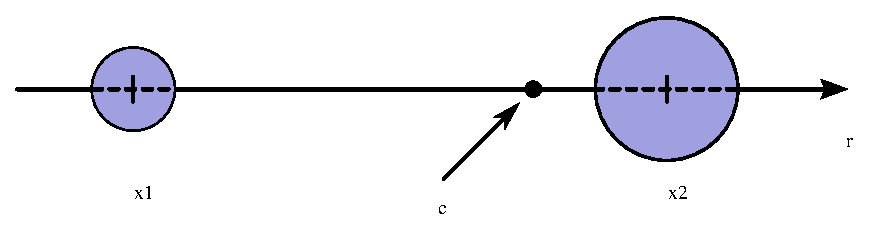
\includegraphics[height=1.8cm]{Figures/6Chapter/mass}
\end{psfrags}
\end{center}
\caption{The center of mass on the figure is indicated by the tip of the arrow.
In general, the mean of a random variable corresponds to the center of mass of the associated particle system}
\end{figure}
\end{example}


\subsection{The Variance}

A second widespread descriptive quantity associated with random variable $X$ is its \emph{variance}, which we denote by $\Var [X]$. \index{Variance}
It is defined by
\begin{equation} \label{equation:VarianceExplicit}
\Var [X] = \Expect \left[ \left( X - \Expect [X] \right)^2 \right] .
\end{equation}
Evidently, the variance is always nonnegative.
It provides a measure of the dispersion of $X$ around its mean.
For discrete random variables, it can be computed explicitly as
\begin{equation*}
\Var [X] = \sum_{x \in X(\Omega)} \left( x - \Expect [X] \right)^2 p_X (x) .
\end{equation*}
The square root of the variance is referred to as the \emph{standard deviation} of $X$, and it is often denoted by $\sigma$. \index{Standard deviation}

\begin{example}
Suppose $X$ is a Bernoulli random variable with parameter $p$.
We can compute the mean of $X$ as
\begin{equation*}
\Expect [X] = 1 \cdot p + 0 \cdot (1 - p) = p .
\end{equation*}
Its variance is given by
\begin{equation*}
\Var [X] = (1 - p)^2 \cdot p + (0 - p)^2 \cdot (1 - p)
= p (1 - p) .
\end{equation*}
\end{example}

\begin{example} \label{example:PoissonMeanVariance}
Let $X$ be a Poisson random variable with parameter $\lambda$.
The mean of $X$ is given by
\begin{equation*}
\begin{split}
\Expect [X] &= \sum_{k=0}^{\infty} k \frac{\lambda^k}{k!} e^{- \lambda}
= \sum_{k=1}^{\infty} \frac{\lambda^k}{(k-1)!} e^{- \lambda} \\
&= \lambda \sum_{\ell=0}^{\infty} \frac{\lambda^\ell}{\ell!} e^{- \lambda}
= \lambda .
\end{split}
\end{equation*}
The variance of $X$ can be calculated as
\begin{equation*}
\begin{split}
\Var [X] &= \sum_{k=0}^{\infty} \left( k - \lambda \right)^2
\frac{\lambda^k}{k!} e^{- \lambda} \\
&= \sum_{k=0}^{\infty} \left(\lambda^2 + k (1 - 2 \lambda) + k(k-1) \right)
\frac{\lambda^k}{k!} e^{- \lambda} \\
%&= \lambda^2 + \lambda (1 - 2 \lambda)
%+ \sum_{k=0}^{\infty} k(k-1) \frac{\lambda^k}{k!} e^{- \lambda} \\
&= \lambda - \lambda^2
+ \sum_{k=2}^{\infty} \frac{\lambda^k}{(k-2)!} e^{- \lambda}
%&= \lambda - \lambda^2 +
%\lambda^2 \sum_{m=0}^{\infty} \frac{\lambda^m}{m!} e^{- \lambda}
= \lambda .
\end{split}
\end{equation*}
Both the mean and the variance of a Poisson random variable are equal to its parameter $\lambda$.
\end{example}


\subsection{Affine Functions}

\begin{proposition}
Suppose $X$ is a random variable with finite mean.
Let $Y$ be the affine function of $X$ defined by $Y = aX + b$, where $a$ and $b$ are fixed real numbers.
The mean of random variable $Y$ is equal to $\Expect [Y] = a \Expect [X] + b$.
\end{proposition}
\begin{proof}
This can be computed using \eqref{equation:DiscreteExpectation};
\begin{equation*}
\begin{split}
\Expect [Y] &= \sum_{x \in X(\Omega)} (ax + b) p_X(x) \\
&= a \sum_{x \in X(\Omega)} x p_X(x) + b \sum_{x \in X(\Omega)} p_X(x) \\
&= a \Expect [X] + b.
\end{split}
\end{equation*}
We can summarize this property as $\Expect [a X + b] = a \Expect [X] + b$.
\end{proof}

It is not much harder to show that the expectation is a linear functional.
Suppose that $g(\cdot)$ and $h(\cdot)$ are two real-valued functions such that $\Expect [g(X)]$ and $\Expect [h(X)]$ both exist.
We can write the expectation of $a g(X) + h(X)$ as
\begin{equation*}
\begin{split}
\Expect [ a g(X) + h(X) ] &= \sum_{x \in X(\Omega)} (a g(x) + h(x)) p_X(x) \\
&= a \sum_{x \in X(\Omega)} g(x) p_X(x) + \sum_{x \in X(\Omega)} h(x) p_X(x) \\
&= a \Expect [g(X)] + \Expect [h(X)] .
\end{split}
\end{equation*}
This demonstrates that the expectation is both homogeneous and additive.

\begin{proposition}
Assume that $X$ is a random variable with finite mean and variance, and let $Y$ be the affine function of $X$ given by $Y = aX + b$, where $a$ and $b$ are constants.
The variance of $Y$ is given by $\Var [Y] = a^2 \Var [X]$.
\end{proposition}
\begin{proof}
Consider \eqref{equation:VarianceExplicit} applied to $Y = aX + b$,
\begin{equation*}
\begin{split}
\Var [Y]
&= \sum_{x \in X(\Omega)} \left( ax + b - \Expect [aX + b] \right)^2 p_X(x) \\
&= \sum_{x \in X(\Omega)} \left( ax + b - a \Expect [X] - b \right)^2 p_X(x) \\
&= a^2 \sum_{x \in X(\Omega)} \left( x - \Expect [X] \right)^2 p_X(x)
= a^2 \Var [X] .
\end{split}
\end{equation*}
The variance of an affine function only depends on the distribution of its argument and parameter $a$.
A translation of the argument by $b$ does not affect the variance of $Y = aX + b$.
\end{proof}


\section{Moments}

The \emph{moments} of a random variable $X$ are likewise important quantities used in providing partial information about the PMF of $X$. \index{Moments}
The $n$th moment of random variable $X$ is defined by
\begin{equation} \label{equation:DiscreteMoments}
\Expect [X^n] = \sum_{x \in X(\Omega)} x^n p_X (x) .
\end{equation}
The mean of random variable $X$ is its first moment.

\begin{proposition}
The variance of random variable $X$ can be expressed in terms of its first two moments,
$\Var [X] = \Expect \left[ X^2 \right] - \left( \Expect [X] \right)^2$.
\end{proposition}
\begin{proof}
Suppose that the variance of $X$ exists and is finite.
Starting from \eqref{equation:VarianceExplicit}, we can expand the variance of $X$ as follows,
\begin{equation*}
\begin{split}
\Var [X] &= \sum_{x \in X(\Omega)} \left( x - \Expect [X] \right)^2 p_X (x) \\
&= \sum_{x \in X(\Omega)} \left( x^2 - 2 x \Expect [X] + \left( \Expect [X] \right)^2 \right) p_X (x) \\
&= \sum_{x \in X(\Omega)} x^2 p_X (x) - 2 \Expect [X] \sum_{x \in X(\Omega)} x p_X (x) + \left( \Expect [X] \right)^2 \sum_{x \in X(\Omega)} p_X (x) \\
&= \Expect \left[ X^2 \right] - \left( \Expect [X] \right)^2.
\end{split}
\end{equation*}
This alternate formula is sometimes convenient for computational purposes.
\end{proof}

We offer below an example where the above formula for the variance is applied.
This allows the application of standard sums from calculus.

\begin{example}
Let $X$ be a uniform random variable with PMF
\begin{equation*}
p_X (k) = \left\{ \begin{array}{ll}
1/n, & \text{if }k = 1, 2, \ldots, n \\
0, & \text{otherwise} .
\end{array} \right.
\end{equation*}
The mean of this uniform random variable is equal to
\begin{equation*}
\Expect [X] = \frac{n+1}{2} .
\end{equation*}
The variance of $X$ can be obtained as
\begin{equation*}
\begin{split}
\Var [X] &= \Expect \left[ X^2 \right] - \left( \Expect [X] \right)^2
= \sum_{k=1}^n \frac{k^2}{n} - \left( \frac{n+1}{2} \right)^2 \\
&= \frac{n(n+1)(2n+1)}{6n} - \left( \frac{n+1}{2} \right)^2 \\
%&= \frac{2n^2 + 3n + 1}{6} - \frac{n^2 + 2n + 1}{4} \\
%&= \frac{4n^2 + 6n + 2}{12} - \frac{3n^2 + 6n + 3}{12} \\
&= \frac{n^2 - 1}{12} .
\end{split}
\end{equation*}
\end{example}

Closely related to the moments of a random variable are its \emph{central moments}. \index{Central moments}
The $k$th central moment of $X$ is defined by $\Expect \left[ \left( X - E[X] \right)^k \right]$.
The variance is an example of a central moment, as we can see from definition \eqref{equation:VarianceExplicit}.
The central moments are used to define the \emph{skewness} of random variable, which is a measure of asymmetry; and its \emph{kurtosis}, which assesses whether the variance is due to infrequent extreme deviations or more frequent, modest-size deviations.
Although these quantities will not play a central role in our exposition of probability, they each reveal a different characteristic of a random variable and they are encountered frequently in statistics. 


\section{Ordinary Generating Functions}
\label{section:OrdinaryGeneratingFunctions}

In the special yet important case where $X(\Omega)$ is a subset of the non-negative integers, it is occasionally useful to employ the \emph{ordinary generating function}. \index{Ordinary generating function}
This function bears a close resemblance to the \emph{$z$-transform} and is defined by \index{$z$-transform}
\begin{equation} \label{equation:OrdinaryGeneratingFunction}
G_X(z) = \Expect \left[ z^X \right] = \sum_{k=0}^{\infty} z^k p_X (k) .
\end{equation}
It is also called the \emph{probability-generating function} because of the following property. \index{Probability-generating function}
The probability $\Pr (X = k) = p_X(k)$ can be recovered from the corresponding generating function $G_X (z)$ through Taylor series expansion.
Within the radius of convergence of $G_X(z)$, we have
\begin{equation*}
G_X(z) = \sum_{k=0}^{\infty} \frac{1}{k!} \left( \frac{d^k G_X}{dz^k}(0) \right) z^k .
\end{equation*}
Comparing this equation to \eqref{equation:OrdinaryGeneratingFunction}, we conclude that
\begin{equation*}
p_X(k) = \frac{1}{k!} \frac{d^k G_X}{dz^k} (0) .
\end{equation*}
We note that, for $|z| \leq 1$, we have
\begin{equation*}
\left| \sum_{k=0}^{\infty} z^k p_X(k) \right|
\leq \sum_{k=0}^{\infty} |z|^k p_X(k)
\leq \sum_{k=0}^{\infty} p_X(k) = 1
\end{equation*}
and hence the radius of convergence of any probability-generating function must include one.

The ordinary generating function plays an important role in dealing with sums of discrete random variables.
As a hint of what lies ahead, we compute ordinary generating functions for Bernoulli and Binomial random variables below.

\begin{example}
Let $X$ be a Bernoulli random variable with parameter $p$.
The ordinary generating function of $X$ is given by
\begin{equation*}
G_X(z) = p_X(0) + p_X(1) z
= 1 - p + pz .
\end{equation*}
\end{example}

\begin{example}[Binomial random variable]
Let $S$ be a binomial random variable with parameters $n$ and $p$.
The ordinary generating function of $S$ can be computed as
\begin{equation*}
\begin{split}
G_S(z) &= \sum_{k=0}^{n} z^k p_S (k)
= \sum_{k=0}^{n} z^k \binom{n}{k} p^k (1 - p)^{n-k} \\
&= \sum_{k=0}^{n} \binom{n}{k} (pz)^k (1 - p)^{n-k}
= (1 - p + pz)^n .
\end{split}
\end{equation*}
\end{example}

We know, from Section~\ref{subsection:BinormialRandomVariables}, that one way to create a binomial random variable is to sum $n$ independent and identically distributed Bernoulli random variables, each with parameter $p$.
Looking at the ordinary generating functions above, we notice that the $G_S(z)$ is the product of $n$ copies of $G_X(z)$.
Intuitively, it appears that the sum of independent discrete random variables leads to the product of their ordinary generating functions, a fact that we will be checking shortly.

The mean and second moment of $X$ can be computed based on its ordinary generating function,
In particular, we have
\begin{equation*}
\Expect [X] = \lim_{z \uparrow 1} \frac{d G_X}{dz}(z) .
\end{equation*}
Similarly, the second moment of $X$ can be derived as
\begin{equation*}
\Expect \left[ X^2 \right]
= \lim_{z \uparrow 1} \left( \frac{d^2 G_X}{dz^2}(z) + \frac{d G_X}{dz}(z) \right) .
\end{equation*}
This can be quite useful, as seen in the following example.

\begin{example}[Poisson Random Variable]
Suppose that $X$ has a Poisson distribution with parameter $\lambda > 0$.
The function $G_X(s)$ is computed using the distribution of $X$,
\begin{equation*}
G_X(z) = \sum_{k = 0}^\infty z^{k} \frac{e^{-\lambda}\lambda^k}{k!}
= e^{-\lambda} \sum_{k = 0}^\infty \frac{(\lambda z)^k}{k!}
= e^{-\lambda} e^{\lambda z} = e^{\lambda(z - 1)} .
\end{equation*}
The first two moments of $X$ are given by
\begin{align*}
\Expect [X] &= \lim_{z \uparrow 1} \frac{d G_X}{dz} (z)
= \lim_{z \uparrow 1} \lambda e^{\lambda(z - 1)} = \lambda \\
\Expect \left[ X^2 \right] &= \lim_{z \uparrow 1}
\left( \frac{d^2 G_X}{dz^2} (z) + \frac{d G_X}{dz} (z) \right)
= \lim_{z \uparrow 1} \left( \lambda^2 + \lambda \right)
e^{\lambda (z - 1)} = \lambda^2 + \lambda .
\end{align*}
This provides a very efficient way to compute the mean and variance of $X$, which are both equal to $\lambda$.
Compare this method with Example~\ref{example:PoissonMeanVariance}.
\end{example}


\section*{Further Reading}

\begin{small}
\begin{enumerate}
\item Ross, S., \emph{A First Course in Probability}, 7th edition, Pearson Prentice Hall,2006: Section~4.3.
\item Bertsekas, D.P., and Tsitsiklis, J.N., \emph{Introduction to Probability}, Athena Scientific, 2002: Section~2.4.
\end{enumerate}
\end{small}

